\documentclass[11pt]{report}
%Gummi|061|=)
\usepackage[utf8]{inputenc}
\usepackage{graphicx}

\title{\textbf{GIT SCM practices}}
\author{Daniele Bacarella\\Kiril Goguev}
\date{}
\begin{document}

\maketitle

The following is a document that notes how the Erlang backend group will use git when developing the Erlang NetInf Backend. 

\tableofcontents


\chapter{GIT Repository structure and policies}

There will be 4 persistent branches.
\begin{itemize}
\item master
\item staging
\item develop
\item release
\end{itemize}

The following naming convention for temporary branches is adopted: 

\begin{itemize}
\item SprintX.shortStoryName
\end{itemize}



NOTE: ALL story tasks are done in the pair programming paradigm. The temporary branches will be deleted after each successful merge to the DEVELOP branch.

\subsection {Policies}
\begin{itemize}
\item master\\ \\
The 'master' branch will only contain Demo code. This is the code from the backend group which contains ONLY the fully tested and integrated stories.  \\Tags will be made here under the following convention:\\ \emph{SprintX.shortStoryName}\newpage
This is a JENKINS build tool controlled area - No human user should be operating in this branch. \\JENKINS is responsible for  merging from 'master' to 'develop' at the end of a sprint- in order to keep the branches synchronized and provide a fresh clean start for each sprint from working demo code.\\
\item release\\ \\
The 'release' branch will only contain individual stories which are completed and fully unit tested. Here we can pick and choose which stories to include in a specific demo. This branch is also a JENKINS build tool area. \\JENKINS is responsible for integration testing and merging between 'release' and 'master'
\item develop\\ \\
The 'develop' branch will contain all the code this is able to be compiled on the server and is where the human users will start their personal story branches. Also a JENKINS build tool area, The code here will be considered in a "Story done and compiles but not yet tested" state.\\ JENKINS is responsible for unit testing and merging between 'develop' and 'release'

\item staging \\ \\
The 'staging' branch will contain all the dirty code and is where the human users will push all their code when finished for the end of the day. Also a JENKINS Build tool area, the code here will be considered in a story is in progress it may be done but it also may not compile. JENKINS will pull all the code from this branch and try to compile it, if it compiles then it will be merged with the 'develop' branch.

\item SprintX.shortStoryName\\ \\
The branch's name will contain the local working code for the specific sprint story followed by a short story name-typically the name written on the post it note for example: MSG\_Handler. A merge to the DEVLEOP branch will mean the story is considered done for the sprint but requires testing by integration tools and JENKINS. This branch will be deleted after the tests are passed and the a successful merge is complete. History will be kept in the 'develop' branch should we need to revert for any reason. 
\end{itemize}


\chapter{Naming conventions}
Where ever possible, the JENKINS build tool will be configured to create the branches and tags accordingly. 
\subsection{Branches}
With the exception of the RELEASE and the MASTER, each branch will be labelled as follows: SprintX.StoryY -where X is the sprint number and Y is the Story number
\subsection{Tags}
There will be at least 2 places in the GIT repository where we will use tags.
\begin{enumerate}
\item master
\item release
\end{enumerate}
Each tag will be labelled as follows SprintX.shortStoryName-RELEASE or SprintX-DemoZ depending on the sprint and which branch is being pushed to.


\chapter{Sample work flow}

The following section will detail a sample work flow for a sprint with at least two story items. 

The follow image can quickly show you how the individual story may look on a time-line.
\begin{figure}[htb]
\centering
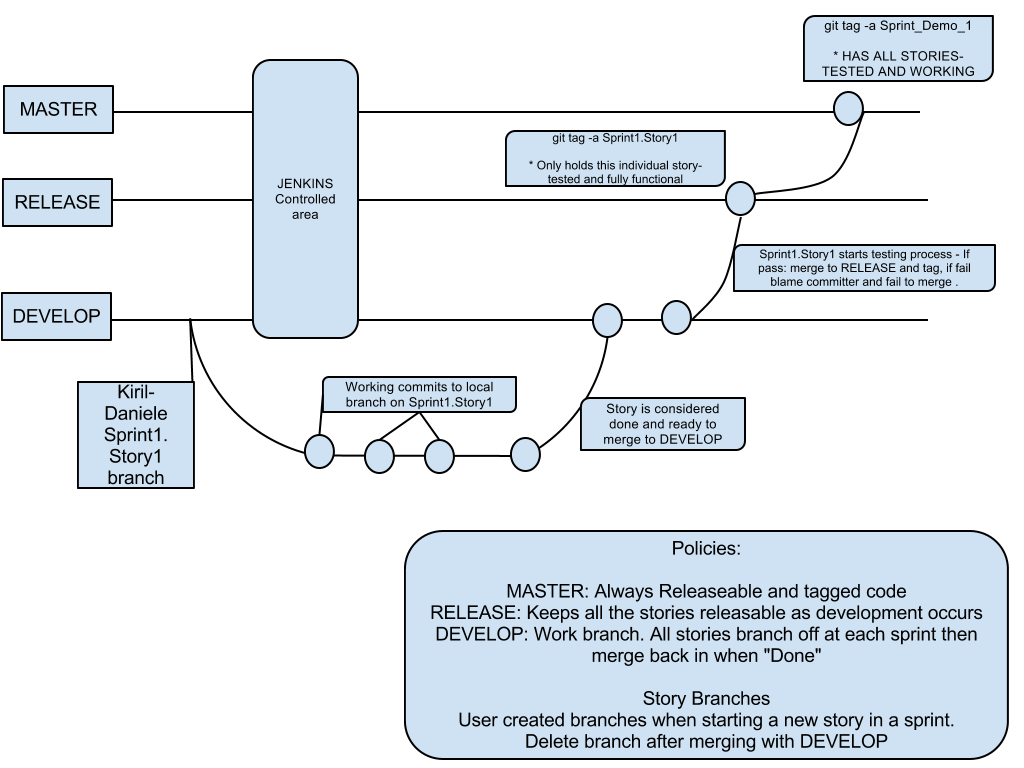
\includegraphics[width=1\textwidth]{workflow}
\caption{Sample workflow for one story item}
\label{fig:architecture}
\end{figure}


\subsection{Starting a sprint}

At the start of each sprint the development team will perform a git checkout -b SprintX.shortStoryName DEVELOP

for a running example we will take the HTTP Handler from the first sprint. 
\begin{verbatim}
git checkout -b SprintX.shortStoryName develop
git push -u origin SprintX.shortStoryName
\end{verbatim}
This will pull all the previous items into your temporary working branch from develop

\subsection{Working during a sprint}

As you and your partner work together to complete the tasks outlined in the story, commit as usual to your local branch.\\
\begin{verbatim}
git pull origin staging
git add [files that have been added or created/modified]
git commit -m description - where description is the commit message you would like associated with the commit. 
\end{verbatim}
\subsection{Deploying a Done story}

After all the tasks are completed and you feel ready to move the task to the DONE state, merge it to the development branch using the following command:\\

\begin{verbatim}
git checkout staging
git merge --no-ff SprintX.shortStoryName
git push origin staging


- do the following only if you wish to delete your branch on the remote repository -
git push origin :SprintX.shortStoryName

- do the following if you wish to delete your branch locally -  
git branch -d SprintX.shortStoryName
\end{verbatim}
This will perform a merge and fast-forward on the remote 'staging' branch while keeping historical information.
This will also create empty commits in the development branch as a way to quickly spot revisions which you may wish to go back to, for example if you need to remove a story that was not working properly.
\newpage
\textbf {NOTE: AS A HUMAN USER THIS IS TYPICALLY WHERE YOU STOP WORKING IN THE WORKFLOW. \\THE FOLLOWING STEPS ARE TO BE IMPLEMENTED BY JENKINS AND AUTOMATED BUILD TOOLS. YOU ARE ONLY CONCERNED WITH WORKING ON THE DEVELOP BRANCH AND YOUR OWN STORY BRANCHES FOR EACH SPRINT. YOU SHOULD NEVER TOUCH MASTER OR RELEASE UNLESS ABSOLUTELY NECESSARY}

\subsection{Testing a sprint story}

The following steps assume that a testing suite was created and works well with JENKINS build tool. 

\subsection{Merging in to develop}
As a story branch has been merged to 'develop', the code goes through a set of unit tests and when it successfully passes all of them, it is ready to be merged to 'release': 
\begin{verbatim}
git checkout develop
git merge --no-ff staging
git push origin develop
\end{verbatim}

\subsection{Merging in to release}
As a story branch has been merged to 'develop', the code goes through a set of unit tests and when it successfully passes all of them, it is ready to be merged to 'release': 
\begin{verbatim}
git checkout release
git merge --no-ff develop
git tag -a SprintX.shortStoryName-RELEASE
git push origin release
\end{verbatim}
\subsection{Merging in to master}
Supposing that all the sprint stories code have reached the stage of release, before proceeding with the final merging , we check that all the desired features have been implemented and tested properly.
The final merging is performed upon the MASTER branch containing always the stable version of all the code written so far.
  \begin{verbatim}
git checkout master
git merge --no-ff release
git tag -a Sprint1.Demo1
git push origin master
\end{verbatim}
\subsection{Post-sprint practice}

After each sprint we should synchronize the 'master' and the 'develop' branch. This ensures a clean start for each sprint as the 'staging' branch will inherently be considered the "dirty" branch. 

  \begin{verbatim}
git checkout DEVELOP
git merge --no-ff MASTER
\end{verbatim}

\chapter{References}
The following was an inspiration for the git model:\\

http://nvie.com/posts/a-successful-git-branching-model/

\end{document}
